\section{Results}
\begin{itemize}
 \item In this section you should have all the figures and tables.
 \item Please ensure that the report shows your figures and tables exactly where you originally intended it to be. 
 The package called \textit{Float} is quite useful for this purpose. 
 \item Please check that your figures and tables contain \textbf{title, and caption}.
 \item Graphs of any kind should have their axes explicitly defined by you.  Also please mention the unit of measurement and keep the tick values of graphs.
 \item If 2 or more figures are to be compared then please ensure that they are in the \underline{same scale}, for not just the benefit of your TAs and instructors, but
 also your own benefit to visualize and interpret your results better.
 \item If your figure contains colour codes, please use \underline{legends} and \underline{colorbars} to help the reader.
\end{itemize}
\begin{figure}[H]
\centering
   
\includegraphics[width=0.5\textwidth]{workClean.png}
   \caption{This figure lacks the axes tick labels and units of measurement. We kindly request you to provide not just axes labels but also axes measurements and units of measurements.}
   \label{fig:noTicks}
\end{figure}
Humour aside, please also avoid the following.
\begin{figure}[H]
\centering
   
\includegraphics[width=0.5\textwidth]{pageLimit.png}
   \caption{Please try neither. If your figure size is so small that the readability and resolution are compromised, then so shall your grades be. If you have been able to keep your report concise
   and yet been able to describe what you wanted to tell then keep it like that.}
   \label{fig:PageLimit}
\end{figure}
If the titles and axes labels are not readable, they will be considered as absent. 

\begin{figure}[h]
\begin{center}
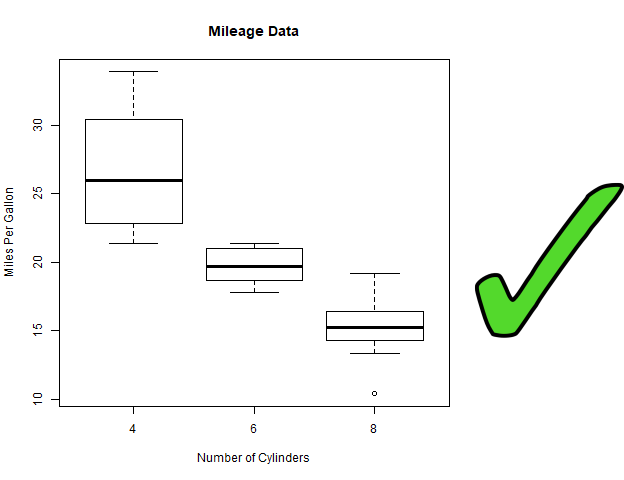
\includegraphics[width=0.5\textwidth]{boxplot}
\caption{Boxplot example from mtcars data.}
\label{fig:rboxplot}
\end{center}
\end{figure}
Figure \ref{fig:rboxplot} was created by the script from tutorialspoint \cite{Rboxplot}. The above is given as an example of an ideal figure. Notice how it contains proper and visible axes, axes labels, 
captions, and title. The figure has good resolution. Produce figures of such quality (with respect to resolution, axes information, label information, units, etc).